\subsection{Well management service}

\subsubsection{Overview}

The \texttt{WellManagementService} is a service component responsible for handling well configuration requests and building appropriate well models for simulation. It processes requests containing well specifications, constructs wells based on various templates (I-well, J-well, S-well, H-well), and returns a response with simulation-ready well models.

\subsubsection{Architecture}

The well management subsystem follows a layered architecture with clear separation of concerns.

\begin{itemize}
	\item \texttt{WellManagementService}
	\item \texttt{WellTemplateInterface} (Abstract)
	\begin{itemize}
		\item \texttt{IWellTemplate} (Vertical well)
		\item \texttt{JWellTemplate} (J-shaped well)
		\item \texttt{SWellTemplate} (S-shaped well)
		\item \texttt{HWellTemplate} (Horizontal well)
	\end{itemize}
	\item \texttt{SectionInterface} (Abstract)
	\begin{itemize}
		\item \texttt{LinearWellSection}
		\item \texttt{CurvedWellSection}
	\end{itemize}
	\item \texttt{WellBuilder}
	\item Support classes:
	\begin{itemize}
		\item \texttt{PerforationMdProvider}
		\item \texttt{PerforationRange}
	\end{itemize}
\end{itemize}

This architecture provides several benefits:
\begin{itemize}
	\item \textbf{Separation of Concerns}: Each component has a specific, focused responsibility.
	\item \textbf{Extensibility}: New well types can be added by creating new templates without modifying existing code.
	\item \textbf{Maintainability}: The builder pattern isolates construction logic, making it easier to update.
	\item \textbf{Testability}: Components can be tested in isolation with appropriate mocks.
\end{itemize}

\begin{figure}[H]
	\centering
	\includesvg[width=1.0\textwidth]{content/images/WellManagementServiceUML}
	\caption{Well management service system UML}
	\label{fig:WellManagementServiceUML}
\end{figure}


\subsubsection{System components}
\begin{itemize}
	\item \textbf{WellManagementService}: Acts as a facade for the subsystem, receiving JSON requests, coordinating the creation of wells, and returning standardized responses.

	\item \textbf{Well Templates}: Specialized factories for different well types (I-well, J-well, S-well, H-well) that encapsulate the configuration logic specific to each well geometry.

	\item \textbf{WellBuilder}: Implements the builder pattern to provide a fluent interface for constructing complex well objects with various configurations.

	\item \textbf{Well Models}: Data structures representing wells and their properties, used both for input configuration and output results.
\end{itemize}

The flow of data through the system is as follows:

\begin{enumerate}
	\item Client sends a request with well configurations to the WellManagementService.
	\item The service parses the request and identifies the well types needed.
	\item For each well configuration, the appropriate template is selected and used.
	\item Templates configure WellBuilder instances with the correct geometrical properties.
	\item WellBuilder constructs complete Well objects with the specified properties.
	\item Wells are converted to SimulationWellModels for the response.
	\item The service returns a standardized response with the constructed wells.
\end{enumerate}


\subsubsection{Public API}

	\begin{verbatim}
		process_request(request_dict: dict[str, Any]) -> WellManagementServiceResponse
	\end{verbatim}

Main entry point for the service. Processes a dictionary representation of a well management request.

\begin{itemize}
	\item \textbf{Parameters:}
	\begin{itemize}
		\item \texttt{request\_dict}: Dictionary containing well specification data
	\end{itemize}
	\item \textbf{Returns:}
	\begin{itemize}
		\item \texttt{WellManagementServiceResponse}: Object containing processed simulation well models
	\end{itemize}
	\item \textbf{Description:}\\
	This method parses the input dictionary into a \texttt{WellManagementServiceRequest} object, logs the parsed request for debugging purposes, and delegates to the private \texttt{\_build\_wells} method to generate the wells based on the request configuration. The final result is a \texttt{WellManagementServiceResponse} containing simulation-ready well models.
\end{itemize}

\begin{verbatim}
dump_results_schema(path: Path | str) -> None
\end{verbatim}


Generates and saves the JSON schema for the service response.

\begin{itemize}
\item \textbf{Parameters:}
\begin{itemize}
\item \texttt{path}: File path (as string or Path object) where the schema will be saved
\end{itemize}
\item \textbf{Returns:}
\begin{itemize}
\item None
\end{itemize}
\item \textbf{Description:}\\
This method generates the JSON schema for the \texttt{WellManagementServiceResponse} class and writes it to the specified path. This schema documentation can be used by clients to understand the structure of the service response.
\end{itemize}



\subsubsection{Data Models Schema}

\textbf{PerforationRangeModel}
\begin{figure}[H]
	\begin{lstlisting}[language=Python, caption=PerforationRangeModel class definition]
		class PerforationRangeModel(BaseModel):
		start_md: float
		end_md: float
	\end{lstlisting}
\end{figure}

Defines a perforation range in measured depth along a wellbore.

\begin{itemize}
	\item \textbf{Attributes:}
	\begin{itemize}
		\item \texttt{start\_md}: Starting measured depth of the perforation
		\item \texttt{end\_md}: Ending measured depth of the perforation
	\end{itemize}
	\item \textbf{Validation:}
	\begin{itemize}
		\item Ensures that \texttt{start\_md} is less than \texttt{end\_md}
	\end{itemize}
\end{itemize}

\textbf{PositionModel}
\begin{figure}[H]
	\begin{lstlisting}[language=Python, caption=PositionModel class definition]
		class PositionModel(BaseModel):
		x: float
		y: float
		z: float
	\end{lstlisting}
\end{figure}

Represents a 3D coordinate position.

\begin{itemize}
	\item \textbf{Attributes:}
	\begin{itemize}
		\item \texttt{x}: X-coordinate
		\item \texttt{y}: Y-coordinate
		\item \texttt{z}: Z-coordinate
	\end{itemize}
\end{itemize}

\textbf{IWellModel}
\begin{figure}[H]
	\begin{lstlisting}[language=Python, caption=IWellModel class definition]
		class IWellModel(BaseModel):
		well_type: Literal["I"] = "I"
		name: str
		md: float
		wellhead: tuple[float, float, float]
		md_step: float = Field(ge=0.1)
		perforations: list[PerforationRangeModel] = []
	\end{lstlisting}
\end{figure}

Represents a vertical (I-type) well.

\begin{itemize}
	\item \textbf{Attributes:}
	\begin{itemize}
		\item \texttt{well\_type}: Fixed as "I" to identify the well type
		\item \texttt{name}: Name of the well
		\item \texttt{md}: Maximum measured depth (total length) of the well
		\item \texttt{wellhead}: 3D coordinates of the wellhead (starting point)
		\item \texttt{md\_step}: Discretization step size along the well (must be greater than or equal to 0.1)
		\item \texttt{perforations}: List of perforation ranges along the well (default: empty list)
	\end{itemize}
\end{itemize}

\textbf{JWellModel}
\begin{figure}[H]
	\begin{lstlisting}[language=Python, caption=JWellModel class definition]
		class JWellModel(BaseModel):
		well_type: Literal["J"] = "J"
		name: str
		md_linear1: float
		md_curved: float
		dls: float
		md_linear2: float
		wellhead: tuple[float, float, float]
		azimuth: float = 0.0
		md_step: float = Field(ge=0.1)
		perforations: list[PerforationRangeModel] = []
	\end{lstlisting}
\end{figure}

Represents a J-shaped well with one curved section.

\begin{itemize}
	\item \textbf{Attributes:}
	\begin{itemize}
		\item \texttt{well\_type}: Fixed as "J" to identify the well type
		\item \texttt{name}: Name of the well
		\item \texttt{md\_linear1}: Measured depth of the first (vertical) linear section
		\item \texttt{md\_curved}: Measured depth of the curved section
		\item \texttt{dls}: Dogleg severity (rate of change in angle) in degrees per unit length
		\item \texttt{md\_linear2}: Measured depth of the second (deviated) linear section
		\item \texttt{wellhead}: 3D coordinates of the wellhead (starting point)
		\item \texttt{azimuth}: Azimuth angle in degrees (default: 0.0)
		\item \texttt{md\_step}: Discretization step size along the well (must be greater than or equal to 0.1)
		\item \texttt{perforations}: List of perforation ranges along the well (default: empty list)
	\end{itemize}
\end{itemize}

\textbf{SWellModel}
\begin{figure}[H]
	\begin{lstlisting}[language=Python, caption=SWellModel class definition]
		class SWellModel(BaseModel):
		well_type: Literal["S"] = "S"
		name: str
		md_linear1: float
		md_curved1: float
		dls1: float
		md_linear2: float
		md_curved2: float
		dls2: float
		md_linear3: float
		wellhead: tuple[float, float, float]
		azimuth: float = 0.0
		md_step: float = Field(ge=0.1)
		perforations: list[PerforationRangeModel] = []
	\end{lstlisting}
\end{figure}

Represents an S-shaped well with two curved sections.

\begin{itemize}
	\item \textbf{Attributes:}
	\begin{itemize}
		\item \texttt{well\_type}: Fixed as "S" to identify the well type
		\item \texttt{name}: Name of the well
		\item \texttt{md\_linear1}: Measured depth of the first (vertical) linear section
		\item \texttt{md\_curved1}: Measured depth of the first curved section
		\item \texttt{dls1}: Dogleg severity for the first curved section in degrees per unit length
		\item \texttt{md\_linear2}: Measured depth of the second (intermediate) linear section
		\item \texttt{md\_curved2}: Measured depth of the second curved section
		\item \texttt{dls2}: Dogleg severity for the second curved section in degrees per unit length
		\item \texttt{md\_linear3}: Measured depth of the third (final) linear section
		\item \texttt{wellhead}: 3D coordinates of the wellhead (starting point)
		\item \texttt{azimuth}: Azimuth angle in degrees (default: 0.0)
		\item \texttt{md\_step}: Discretization step size along the well (must be greater than or equal to 0.1)
		\item \texttt{perforations}: List of perforation ranges along the well (default: empty list)
	\end{itemize}
\end{itemize}

\textbf{HWellModel}
\begin{figure}[H]
	\begin{lstlisting}[language=Python, caption=HWellModel class definition]
		class HWellModel(BaseModel):
		well_type: Literal["H"] = "H"
		name: str
		TVD: float
		md_lateral: float
		wellhead: tuple[float, float, float]
		azimuth: float = 0.0
		md_step: float = Field(ge=0.1)
		perforations: list[PerforationRangeModel] = []
	\end{lstlisting}
\end{figure}

Represents a horizontal well with a vertical section followed by a lateral section.

\begin{itemize}
	\item \textbf{Attributes:}
	\begin{itemize}
		\item \texttt{well\_type}: Fixed as "H" to identify the well type
		\item \texttt{name}: Name of the well
		\item \texttt{TVD}: True vertical depth (vertical section length)
		\item \texttt{md\_lateral}: Measured depth of the lateral (horizontal) section
		\item \texttt{wellhead}: 3D coordinates of the wellhead (starting point)
		\item \texttt{azimuth}: Azimuth angle in degrees (default: 0.0)
		\item \texttt{md\_step}: Discretization step size along the well (must be greater than or equal to 0.1)
		\item \texttt{perforations}: List of perforation ranges along the well (default: empty list)
	\end{itemize}
\end{itemize}

\textbf{WellManagementServiceRequest}
\begin{figure}[H]
	\begin{lstlisting}[language=Python, caption=WellManagementServiceRequest class definition]
		class WellManagementServiceRequest(BaseModel):
		models: list[IWellModel | JWellModel | SWellModel | HWellModel]
	\end{lstlisting}
\end{figure}

Represents a request to the well management service.

\begin{itemize}
	\item \textbf{Attributes:}
	\begin{itemize}
		\item \texttt{models}: List of well models to be processed
	\end{itemize}
\end{itemize}

\textbf{SimulationWellPerforationModel}
\begin{figure}[H]
	\begin{lstlisting}[language=Python, caption=SimulationWellPerforationModel class definition]
		class SimulationWellPerforationModel(BaseModel):
		range: tuple[float, float]
	\end{lstlisting}
\end{figure}

Represents a perforation range in a simulation well model.

\begin{itemize}
	\item \textbf{Attributes:}
	\begin{itemize}
		\item \texttt{range}: Tuple containing the start and end measured depths of the perforation
	\end{itemize}
\end{itemize}

\textbf{WellManagementServiceResponse}
\begin{figure}[H]
	\begin{lstlisting}[language=Python, caption=WellManagementServiceResponse class definition]
		class WellManagementServiceResponse(BaseModel):
		wells: list[SimulationWellModel]
	\end{lstlisting}
\end{figure}

Represents a response from the well management service.

\begin{itemize}
	\item \textbf{Attributes:}
	\begin{itemize}
		\item \texttt{wells}: List of simulation well models generated from the request
	\end{itemize}
\end{itemize}

\subsubsection{Shared models}

Service do not use any shared data models.

\subsubsection{Detailed Workflow}

The \texttt{WellManagementService} provides a comprehensive framework for building and managing various types of well models in petroleum engineering applications. It offers a flexible architecture for creating wells with different geometries including vertical (I-shaped), J-shaped, S-shaped, and horizontal (H-shaped) wells.

The service follows a clear workflow for processing well creation requests:

\begin{enumerate}
	\item Client submits a request containing well specifications
	\item \texttt{WellManagementService.process\_request()} parses the request into a \texttt{WellManagementServiceRequest} object
	\item Service identifies well model types in the request (I, J, S, or H)
	\item For each model, the appropriate template is instantiated
	\item Each template configures and uses a \texttt{WellBuilder} to construct the well
	\item All constructed wells are collected and returned in a \texttt{WellManagementServiceResponse}
\end{enumerate}

The \texttt{WellManagementService} provides a flexible and extensible framework for building various types of well models with different geometries and completions. The architecture leverages design patterns such as Template Method, Builder, and Strategy to create a maintainable and scalable system.


\subsubsection{Dependencies}

\subsubsection{Well models}

	The well model is located in the xz plane as shown on the picture below (note that the z-axis is defined upside down). The LinearWellSection is s fragment of a straight line. Inclination $(\theta)$ is defined as an angle between z-axis and the section. Its values can vary from $-180\degree$ to $180\degree$.

	\begin{figure}[H]
		\centering
		\includegraphics[scale=0.6]{images/well_builder/linear\_section.png}
		\caption{Illustrative drawing of the linear section.}
		\label{linear_section}
	\end{figure}

	The section always starts at the last point in the trajectory (here the coordinate system is centered at that point). If $\theta$ is not provided it is calculated from coordinates of last two points form the trajectory as, such that the section is parallel to the line spanned by these points:
	\begin{equation}
		\theta = \mathrm{atan}\left(\frac{x_{-1} - x_{-2}}{z_{-1} - z_{-2}}\right)
	\end{equation}
	If $z_{-1} - z_{-2} >= 0$, and:
	\begin{equation}
		\theta = \pi + \mathrm{atan}\left(\frac{x_{-1} - x_{-2}}{z_{-1} - z_{-2}}\right)
	\end{equation}
	If the results turns out to be outside of $[-180\degree, 180\degree]$ it needs to be rotated by $-360\degree$.
	\begin{itemize}
		\item $(x_{-1}, z_{-1})$ - coordinates of the last point
		\item $(x_{-2}, z_{-2})$ - coordinates of the second last point
	\end{itemize}

	The curved section is an arc of a circle. It is more complicated than the linear section as in general there are 8 cases. On the picture below the curved sections are shown as starting at the ends of linear sections which are in the trajectory before them. The linear section starting at point (0, 0) is located in one of four quadrants of the coordinate system. In each of these cases the curved segment can curve in 2 directions (clockwise or counter-clockwise). All the cases are shown on the picture below.
	\begin{figure}[H]
		\centering
		\includegraphics[scale=0.4]{images/well_builder/curved\_section.png}
		\caption{Illustrative drawing of the curved section cases.}
		\label{curved_section}
	\end{figure}
	\begin{itemize}
		\item red rods - start points of the curved sections
		\item blue dots - centers of the circles
		\item $\theta$ - inclination
		\item arrows - show direction of curvature
		\item sign of $dls$ encodes information if the start point of the section is on the lower or the upper part of the circle.\\
		$dls > 0$ - start point is on the lower part\\
		$dls < 0$ - start point is on the upper part\\
	\end{itemize}
	In this case inclination is interpreted as the angle between z-axis and the straight line tangent to the trajectory at the start point. If not given it is calculated the same way as it was described in the LinearWellSection. Absolute value of dls is the angle change in degrees over 30 meters of measured distance.\newline

	To determine the trajectory several quantities need to be calculated. These are:
	\begin{itemize}
		\item Circle radius
		\item Angle increase - absolute value of the angular coordinate change in polar coordinates centered on the circle center
		\item Circle center location
		\item Starting point - angular coordinate in polar coordinates centered on the circle center
	\end{itemize}
	Radius is calculated as:
	\begin{equation}
		R = \left|\frac{30} {dls}\right|
	\end{equation}
	where $dls$ is given in radians.\newline
	Angle increase is calculated as:
	\begin{equation}
		\Delta \phi = \frac{md}{R}
	\end{equation}
	Circle center's location is calculated as:
	\begin{equation}
		x_0 = x + sign_x \cdot R \cdot \mathrm{cos}(\theta)
	\end{equation}
	\begin{equation}
		z_0 = z + sign_z \cdot R \cdot \mathrm{sin}(\theta)
	\end{equation}
	\begin{itemize}
		\item $(x_0, z_0)$ - location of the center
		\item $(x, z)$ - location of the starting point
	\end{itemize}
	$sign_x$ and $sign_z$ values are determined by the particular case:

	\begin{itemize}
		\item $sign_x$ = 1 if ($dls >=0$ and $\alpha >= 0$) or ($dls < 0$ and $\alpha < 0$), = -1 otherwise
		\item $sign_z$ = -1 if ($dls >= 0$), = 1 otherwise
	\end{itemize}


	To calculate the angular location of the starting point we introduce parameters:
	\begin{itemize}
		\item $r_x = x - x_0$
		\item $r_z = z - z_0$
	\end{itemize}
	They cannot both be zero as it would mean that the center is in the wellbore.\newline
	The boundary case is $rx=0$. It appears when $\theta = \frac{\pi}{2}$ or $\theta = -\frac{\pi}{2}$. It has subcases:
	\begin{itemize}
		\item $r_x=0$, $r_z<0$: $\phi_{start} = \frac{\pi}{2}$
		\item $r_x=0$, $r_z>0$, $\theta>=0$: $\phi_{start} = -\frac{\pi}{2}$
		\item $r_x=0$, $r_z>0$, $\theta>=0$: $\phi_{start} = \frac{3\pi}{2}$
	\end{itemize}
	$-\frac{\pi}{2}$ and $\frac{3\pi}{2}$ are technically equal. They are treated here separately for computational convenience. To the first one angle increase will be added and from the second one substracted.\newline
	Now we will consider the rest of the cases:
	\begin{itemize}
		\item $r_x>0$, $r_z>0$: $\phi_{start} = -\mathrm{atan}\left(\frac{r_z}{r_x}\right)$
		\item $r_x<0$, $r_z<0$: $\phi_{start} = \pi-\mathrm{atan}\left(\frac{r_z}{r_x}\right)$
		\item $r_x>0$, $r_z<0$: $\phi_{start} = \mathrm{atan}\left(\frac{r_z}{r_x}\right)$
		\item $r_x<0$, $r_z>0$: $\phi_{start} = \pi + \mathrm{atan}\left(\frac{r_z}{r_x}\right)$
	\end{itemize}

	Relation between inclination, dls and curvature direction was presented on the following figure:\\\\
	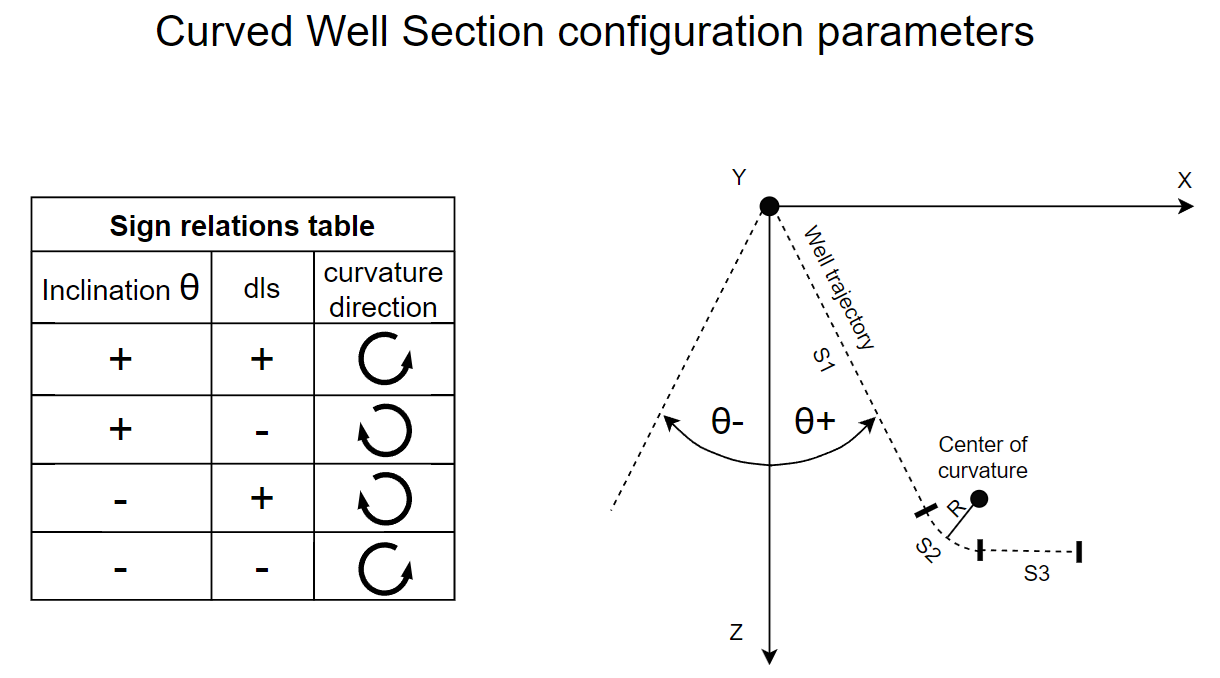
\includegraphics[width=1.0\textwidth]{"images/well_builder/dls_vs_inclination.png"}
